\chapter{Deep Neural Networks for Image Classification: Training, Regularization and Invariance}
\label{chapter:shade}

\renewcommand{\leftmark}{\spacedlowsmallcaps{DNN\textsmaller{s} for Image Classification: Regularization and Invariance}}

\newcommand{\yi}{h}
\newcommand{\Y}{H}
\newcommand{\C}{Y}

\begin{chapabstract}
	{\em
	
    In this chapter, we propose a general overview of the literature regarding the design, training and regularization of \acp{DNN} and \acfp{ConvNet} during the past few years. We discuss recent research directions that will be addressed in this thesis, namely invariance-based regularization, \acf{SSL} and the disentangling of representations.
    %
    In particular, in this chapter, we focus on the question of regularizing \acp{DNN} to make them produce representations that are well fitted for classification and that generalize well on unseen data. A common direction consists in making latent representations encode information that allows to discriminate between the different classes of interest while being invariant to intra-class variations, which are equivalent to noise regarding classification.
    %
    To this end, we propose a regularizer called \acs{SHADE}. This regularization loss is based on a novel idea using information theory metrics to formalize the aforementioned objective of removing the intra-class variance from the latent space. We show that \acs{SHADE} is able to effectively encourages invariance in many standard \acp{ConvNet} architectures and provides an interesting gain over usual baselines on CIFAR-10, as well as studies regarding the behavior of \acp{ConvNet} toward class information.

	\vspace{5mm}
	The work in this chapter, done in collaboration with Michael Blot \citep{blothese}, has led to the publication of a conference paper:}
	\begin{itemize}
		\item \small \fullcite{Blot2018}; best paper award.
	\end{itemize}
\end{chapabstract}

\ifthenelse{\boolean{skipSHADE}}{\endinput}{}

\newpage

\minitoc
\chapterwithfigures{\nameref*{chapter:shade}}
\chapterwithtables{\nameref*{chapter:shade}}

\acresetall

\section{Introduction}

In this chapter, we first propose a general overview of the recent developments in the fields of \acf{DL} and \acfp{ConvNet} used for classification. In particular, we will see how those models are designed, trained and the evolution that allowed those architectures to become the backbone of almost all state-of-the-art models in \ac{CV} research. While our discussion will focus on image classification, it also applies to many semantic tasks of \ac{CV} (detection, segmentation, \etc.).

Key ingredients that make deep \acp{ConvNet} perform so well is their depth and the number of trainable parameters they contain. Having deeper and deeper models with more and more parameters makes it possible to progressively represent more complex decision functions and extract richer and more semantic information from the input images. However, having such complex models comes with an increased risk of overfitting the training set, especially if it contains a small number of images compared to the number of parameters. For example, a ResNet-101 \citep{resnet} model has 44.5M parameters to train while ImageNet contains ``only'' 1.3M images. There is thus a clear unfavorable imbalance between the complexity of our models and the quantity of labeled data at our disposal.

Because of this, finding ways to control the training of \acp{DNN} is a crucial part of the research in \ac{DL}, both to improve their performance on very large datasets but also to eventually be able to train deep architectures on small datasets. To do so, many \textit{regularization} methods have been developed over the years, usually introducing prior human knowledge on desired properties to make the model more robust, such as sparsity of the weights, smoothness of the decision boundary or compression and invariance of the representations.

In this chapter, we investigate in depth this last option and propose a new method to encourage the invariance of the representations. This first contribution, done in collaboration with Michael Blot \citep{blothese}, consists in a new regularization method called {\acs{SHADE}}. Inspired by the \ac{IB} principle \citep{IB} and based on information theory metrics, we propose to minimize the entropy of the representations of a \ac{DNN} conditionally to the class label: $\min \Ent(\Y\mid\C)$. We show that this corresponds to minimizing the intra-class variance of the features, and therefore encourages the construction of features that are intra-class invariant and are thus more fitted for classification. We validate this idea experimentally on various representative \ac{DNN} architectures.

We also introduce interesting directions to improve \acp{DNN} that will be followed in the next chapters. First, the possibility of improving the generalization ability of \acp{DNN} by using additional unlabeled data, which is called \acf{SSL}. This usually consists in finding a method that extracts robust features on labeled and unlabeled data and uses the labeled data to learn the prediction function. Second, through the design of methods that disentangles, \ie separates into independent representations, the different factors of variation of the dataset, greatly increasing the semantic quality of the latent space for various tasks.

In \autoref{shade:sec:RW} we detail the design and training of current deep \acp{ConvNet} and the existing methods to improve their quality. We then present and validate our first contribution, a novel regularization method called \acs{SHADE} in \autoref{shade:sec:model}.


\section{Training and Regularizing Deep Neural Networks} \label{shade:sec:RW}

In this section, we first introduce the general learning framework of \acf{DL} before a focus on the \acf{ConvNet} architectures. We will then go over common techniques to improve the generalization abilities of those models.

\subsection{Deep Learning framework}

\begin{figure}[tb]
	\centering
	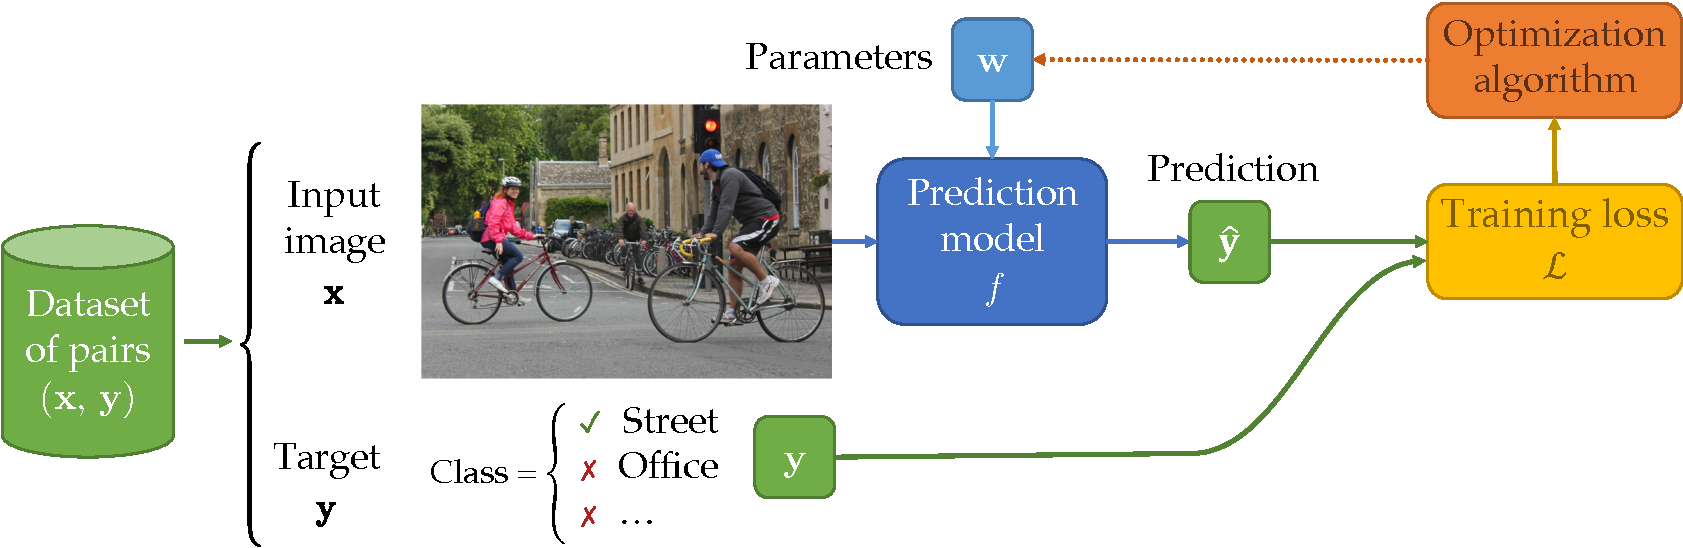
\includegraphics[width=\linewidth]{images/intro_ML}
	\titlecaption{General overview of \acf{ML} training}{Using examples from a dataset, the predictive model learns to make the correct predictions by minimizing a training loss measuring the error made by the model.}
	\label{shade:fig:ML}
\end{figure}

\paragraph{\acf{ML}.} \ac{ML} is a broad domain proposing models that learn to solve a task from examples used to improve themselves. In this thesis, we work mostly on models trained to predict a semantic label. For example, given pictures of cats and dogs, we can learn a model that distinguishes them. Let us go over a typical process used to train an \ac{ML} model, represented by \autoref{shade:fig:ML}.

\ac{ML} proposes to train a \textbf{model} $f$, of \textbf{parameters} $\vw \in \mcW$, taking an input $\vx\in\mcX$ to produce a \textbf{prediction} $\vyh$. Knowing the \textbf{ground-truth label} $\vy \in \mcY$ associated to $\vx$, we can quantify the prediction error of the model by defining a \textbf{loss function} $\mcL_\mathrm{task}(\vyh, \vy)$. Our goal is therefore to find the optimal parameters $\vw^*$ that minimizes the expectation of the loss:
\begin{equation}
	\vw^* = \argmin_\vw \EE_{(\vx, \vy)} \big[\mcL_\mathrm{task}(\vyh, \vy) \big]
  = \argmin_\vw \EE_{(\vx, \vy)} \Big[\mcL_\mathrm{task}\big(f_\vw(\vx), \vy\big) \Big] \,.
\end{equation}

To solve this optimization problem, we use a \textbf{dataset} $\mcD=\{(\vx^{(i)}, \vy^{(i)}), i = 1\dots N_\mathrm{train}\}$ on which we can sample pairs $(\vx, \vy)$ used to estimate the expectation with Monte-Carlo sampling. We then use an \textbf{optimization algorithm} to minimize this empirical loss over the dataset:
\begin{equation}\label{shade:eq:trainnoreg}
	\vw^* = \argmin_\vw \sum_{i=1}^{N_\mathrm{train}} \Big[\mcL_\mathrm{task}\big(f_\vw(\vx^{(i)}), \vy^{(i)}\big) \Big] \,.
\end{equation}

 
\paragraph{\acf{DL}.} \ac{DL} is a subset of \ac{ML} models using \acfp{DNN}, initially inspired by a simple modeling of the neurons proposed by \citet{mcculloch1943logical}. Most of the time, we use \textit{feed-forward} \acfp{NN}, where the model $f$ is a succession (more precisely a directed acyclic graph) of mathematical transformations called \textit{layers} transforming $\vx$ in a succession of \textit{representations} $\vh_\ell$ for each layer $\ell$. The most common layers are \textbf{dense} layers, which consist in a linear transformation of the input $\vh_{\ell} = \vw_\ell \vh_{\ell-1} + b_\ell$; and \textbf{non-linear activation} layers, that can be any function making the model non-linear. Nowadays we mostly use \ac{ReLU} ($\max (0, \vh)$) activation, but hyperbolic tangent ($\tanh$) or sigmoid ($\nicefrac{e^\vh}{e^\vh + 1}$) remain popular options, and many more exist \citep{nwankpa2018activation}. Thanks to their depth, \ie number of layers, \acp{DNN} are able to transform raw input data into more and more complex representations, and thus perform \textit{representation learning} \citep{bengio2013representation}, where the model learns by itself what are the most interesting features to model the input data for the task at hand.

\acfp{NN} are trained using gradient back-propagation \citep{rumelhart1988learning}. This allows to compute progressively, using the chain-rule, the gradient $\nabla_\vw \mcL$ of the loss $\mcL$ with respect to all the weights $\vw$. Using a gradient descent algorithm, we can then update the weights in a direction that decrease the value of the loss, so that progressively, over the course of the training, we finally reach a minimum of the objective function:
\begin{equation}
	\vw \leftarrow \vw - \eta \nabla_\vw \mcL \,.
\end{equation}
Numerous gradient descent algorithms exist, the simplest one being \acf{SGD} \citep{sgd}, with variants designed to improve the speed of the convergence as well as finding a \textit{better} minimum, since \acp{DNN} training losses are non-convex and lots of local minima exist. Famous methods include \ac{SGD} with momentum \citep{rumelhart1988learning}, RMSProp \citep{hinton2012neural}, AdaDelta \citep{duchi2011adaptive} or Adam \citep{adam}.

\subsection{Convolutional architectures}

\begin{figure}[tb]
	\centering
	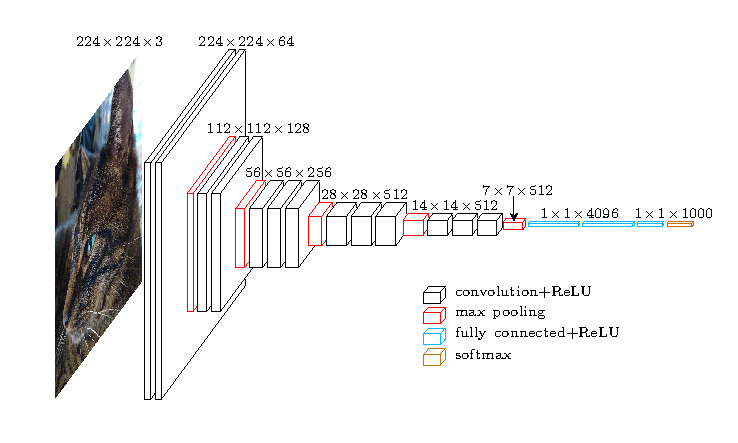
\includegraphics[width=\linewidth]{images/intro_vgg}
	\titlecaption{Architecture of a typical \acs{ConvNet}}{We show the architecture of a VGG-16 \citep{simonyan2015very}, interlacing convolutional layers with max-poolings. \footnotesize{Figure by \citet{vggtibo}.}}
	\label{shade:fig:vgg}
\end{figure}

As we have seen, \acf{DL} became particularly popular for \acf{CV} in 2012 when AlexNet \citep{alexnet} won the \acf{ILSVRC}. This model is a \acf{ConvNet}, a type of \ac{NN} that is specially designed for \ac{CV} tasks. A typical \ac{ConvNet}, such as VGG-16 \citep{simonyan2015very} represented in \autoref{shade:fig:vgg}, is composed of \textbf{convolutional layers} used in place of most or even all of the dense layers of a traditional \ac{DNN}. Indeed, applying a 2D convolution to an image allows to process only small and local patches of information, regardless of their position in the image. Thus, at the beginning of the network, convolutions only look for small patterns in the input image. When going deeper in the network, the use of \textbf{pooling layers} (or by adding stride in a convolution) progressively aggregates the spatial information, bringing closer the information of the patterns found by previous layers. Thus, the next convolutions have a larger receptive field \citep{luo2016understanding} and can assemble the small patterns into bigger and more semantic ones. This behavior of convolutions can be observed by investigating how trained \acp{ConvNet} represent the information, as studied by \citet{olah2017feature} and previously illustrated in \autoref{intro:fig:CNN} (page \pageref{intro:fig:CNN}). We can see that the model first detects contours, assembled into textures, shapes and objects to finally produce the semantic prediction. Interestingly, it can also be noted that the visual cortex is said to work in a similar fashion to this succession of convolutions and pooling \citep{hubel1962receptive}.

\begin{figure}[p]
	\centering
	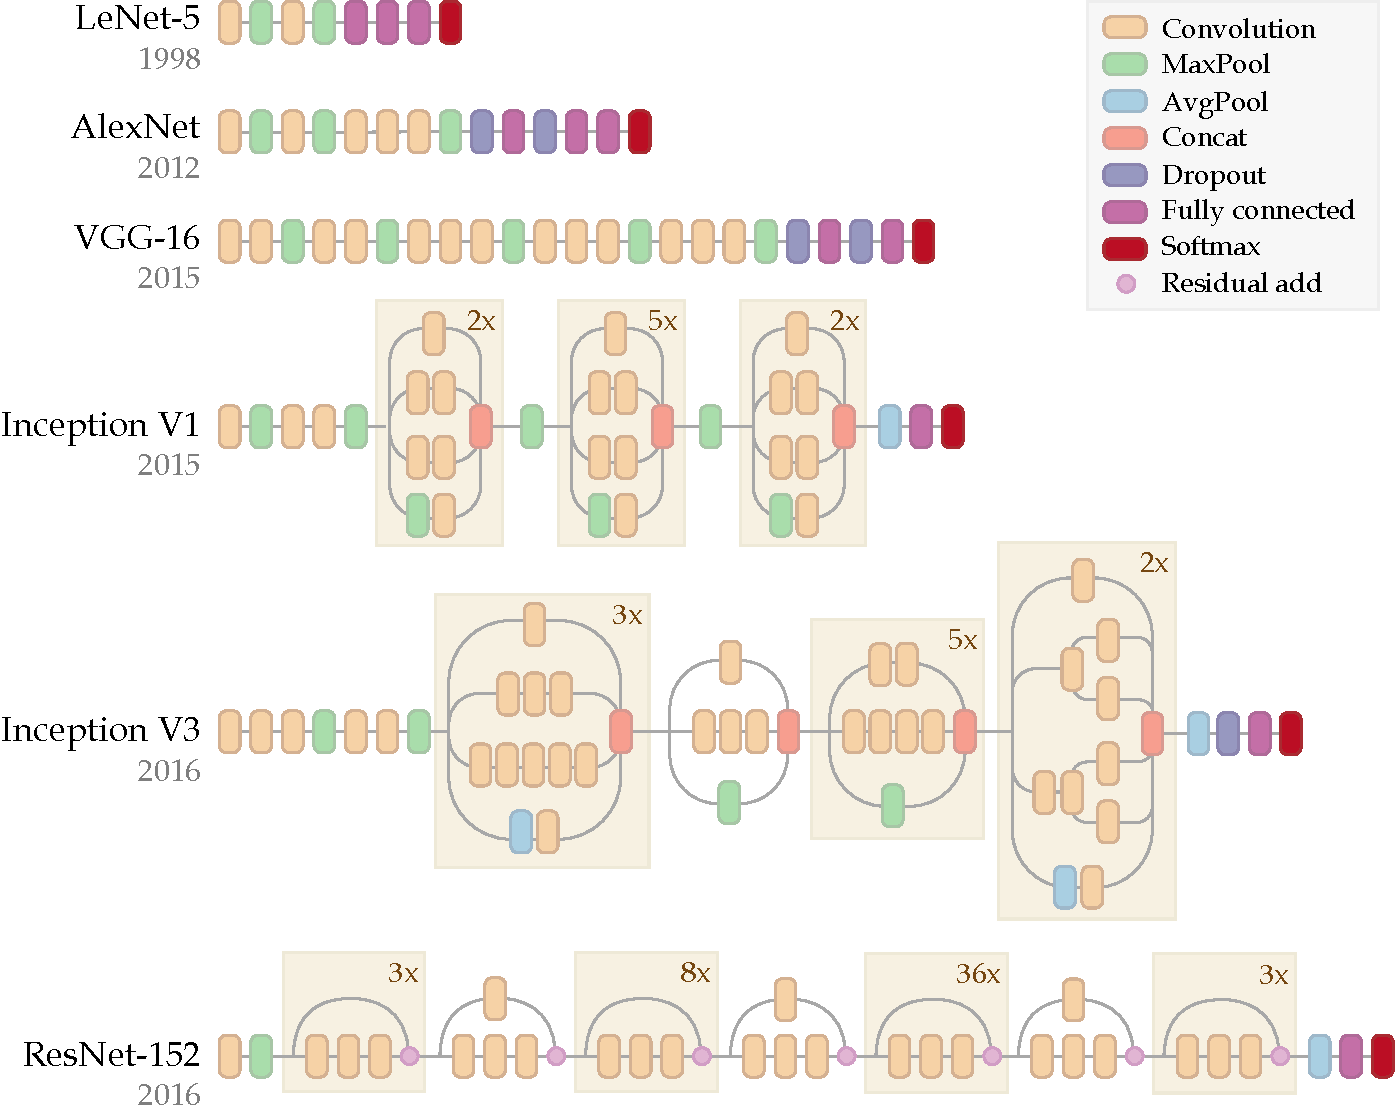
\includegraphics[width=\linewidth]{images/intro_archis}
	\titlecaption[c]{Visualizations of the evolution of standard \acsp{ConvNet} architectures}{over the years. \footnotesize{Style inspired by \citet{googleblog}.}}
	\label{shade:fig:archis}
\end{figure}

\begin{table}[p]
	\centering
	\begin{tabular}{lccc}
		\toprule
		\multirow{2}{*}{Network} & Top-5 error & Number of & Number of \\
		                         & on ImageNet & layers & parameters \\
		\midrule
		AlexNet \citep{krizhevsky2012imagenet} & 16.4\% & 8 & 62M\\
		VGG-16 \citep{simonyan2015very} & 9.3\% & 16 & 138M\\
		Inception V1 \citep{szegedy2015going} & 9.2\% & 22 & 6M\\
		Inception V3 \citep{szegedy2016rethinking} & 5.6\% & 48 & 23M\\
		ResNet-50 \citep{he2016deep} & 6.7\% & 50 & 26M\\
		ResNet-101 \citep{he2016deep} & 6.0\% & 101 & 45M\\
		ResNet-152 \citep{he2016deep} & 5.7\% & 152 & 60M\\
		\bottomrule
	\end{tabular}
	\titlecaption[c]{Overview of popular \ac{ConvNet} architectures}{with their results on ImageNet (\ac{ILSVRC} dataset) in a 10-crop setting (lower than the model ensembling scores submitted to the challenge), along with the number of layers and parameters.}
	\label{shade:fig:ILSVRC}
\end{table}


The first \acp{ConvNet} trained by back-propagation and designed for \ac{CV} dates back decades ago, for example with LeNet-5 \citep{lecun} which classifies handwritten digits. However, as we mentioned, it is only recently that they became the state-of-the-art approach for \ac{CV}. The first notable network is AlexNet \citep{alexnet}, designed to classify natural images of ImageNet \citep{imagenet}, that won \ac{ILSVRC}. In the next years, numerous new \ac{ConvNet} architectures were proposed and won this competition. Popular architectures include VGG-16 \citep{simonyan2015very}, Inception-v1 also called GoogleNet \citep{szegedy2015going} and ResNet \citep{resnet}.

Visualizations of those architectures are presented in \autoref{shade:fig:archis} and their results on ImageNet are presented in \autoref{shade:fig:ILSVRC} for an easy comparison of their architectures. A global trend that we can see is that adding depth to the architecture was one of the key factors for improving the results. Indeed, having more layers allows the model to construct progressively more and more semantically rich features in order to better bridge the ``semantic gap'' between pixels and categories.

As we mentioned, those \ac{ConvNet} architectures we presented have shown to be very versatile regarding the type of \ac{CV} problems they are able to address (classification, detection, segmentation, \acs{VQA}, \etc) and are thus now used as standard building blocks in many \ac{CV} models. This is why we propose to study in depth how those models can be used and improved, first using necessary regularization techniques that allow them to work so efficiently.


\subsection{Regularizing DNNs with priors} \label{shade:sec:RW_regul}

We have seen that \acp{DNN} are trained to find the optimal parameters in order to best predict the labels of the samples in the training dataset $\mcD$. However, a model that perfectly predicts those labels does not necessarily produce the best results on unseen data. For example, if $f_\vw$ can model a very complex function compared to the number of samples in $\mcD$, the model can learn \textit{by heart} the labels $\vy^{(i)}$ associated to $\vx^{(i)}$ without being able to \textbf{generalize} to new samples \citep{vcdim}, which is called \textbf{overfitting}.

Because of their complexity, \ac{DL} models are highly subject to this risk of overfitting the training set while lacking generalization capabilities on the test set. Indeed, they are known to be universal approximators \citep{lu2017expressive} and can possibly produce overly complex decision boundaries. Since the beginning of the development of \acp{DNN}, techniques to control the training of these models were developed.

To overcome this issue, we use \textbf{regularization} which can take multiple forms, a common one being to add a new loss term $\Omega_\mathrm{regul}(\vw,\vx,\vy)$ describing preferred solutions, for example, simpler or smoother decision functions \citep{vapnik1992principles}. Instead of using \autoref{shade:eq:trainnoreg}, we thus have:
\begin{equation}
	\label{shade:eq:train}
	\min_\vw \mcL({\color{greendark}\mcD}, \vw) = \EE_{(\vx, \vy) \in {\color{greendark}\mcD}} \underbrace{\Big[\mcL_\mathrm{task}\big({\color{bluedark}f}_\vw(\vx), \vy\big) + {\color{yellowdark}\Omega_\mathrm{regul}} (\vw,\vx,\vy) \Big]}_{\text{complete loss }\mcL} \,.
\end{equation}

For a model ${\color{bluedark}f}$ of parameters $\vw$, with a dataset ${\color{greendark}\mcD}$ of pairs image-label $(\vx, \vy)$, we try to find the best parameters so as to minimize the target loss $\mcL_\mathrm{task}(\vyh, \vy)$, and using an optional regularization penalty ${\color{yellowdark}\Omega_\mathrm{regul}}$ that can take different forms.
To regularize the training, we can therefore influence:
\begin{itemize}
    \item ${\color{greendark}\mcD}$, by using additional data (\eg \acf{DA}, noise injection, \acf{SSL}\dots);
    \item ${\color{bluedark}f}$, by influencing the architecture of the neural network and introducing layers that can favorably influence its behavior (\eg convolutions, dropout, \acf{BN}\dots);
    \item ${\color{yellowdark}\Omega_\mathrm{regul}}$, by adding loss terms to the optimization objective of the model, to penalize complex models over simpler ones or produce more robust features (\eg weight decay / L2 normalization, invariance and reconstruction costs\dots).
\end{itemize}

\citet{kukavcka2017regularization} present an in-depth review of the techniques used for \acf{DL}. We propose to put into perspective the most important ones in the context of this thesis regarding the improvement of the quality of \acp{DNN}' representations.

Most regularization techniques can have multiple interpretations and have many possible connections with one another \citep[\cf\unskip][chapter 7]{GoodfellowDL}. Here, we organized those methods following the points presented above.
Regularization techniques are usually based on the idea of introducing prior human knowledge of types of models or behaviors that would eventually produce better predictions. Common priors include sparsity (having fewer active parameters or neurons) and smoothness of the decision function, both producing a simpler model that would overfit less; and compression, and invariance which aim at producing features that are more general and correspond to a larger number of examples.

\subsubsection{Using more data}

A first and logical way to improve the quality of the model is to use more data in $\mcD$, directly or indirectly as we will see.

\paragraph{Invariance through \acf{DA}.}
A simple solution to both add invariance to a model and reduce overfitting is to artificially generate new images by producing random variants of existing images of the train set. This is done by changing factors that are considered to have no effect on the semantic content of the image. This technique is called \acf{DA} and is described in details by \citet{dataaugmentation}. In practice, we usually generate a new random variation of each input $\vx$ each time it is used for training. Those random variations can be chosen among a large set of transformations: translations and rotations of the image, horizontal reflection, rescaling (zoom in or out), aspect ratio deformations, selection of random patches in the image, elastic transformations, jittering of the RGB color planes, changes in hue, contrast, brightness, random noise, \etc. This technique is standard for the training of deep \acp{ConvNet} \citep{simard2003best,cirecsan2012multi,alexnet}. For example, for AlexNet, \citet{alexnet} clearly state that \ac{DA} is necessary to train their model. While effective, \ac{DA} has limits, since it produces ``new'' images that are in fact highly correlated to the original images from which they were generated.

Other analogous ideas exist, like \citet{devries2017dataset} who propose to apply the augmentation in the latent space by interpolating and extrapolating between samples' representations; or \citet{goodfellow2014explaining} who propose Adversarial Training, adding to the training set misclassified variations of the input found by gradient descent on the pixels, making the decision function more stable in the neighborhood of existing images.

\paragraph{Noise.}
Adding noise in the training process can be seen as an indirect way to add new artificial data that would be slightly different from the original input \citep{grandvalet1997noise}. It also encourages the model to produce a smooth decision function around existing data points and their representation. Noise can be added to the input \citep{plaut1986experiments}, representations \citep{devries2017dataset}, weights \citep{kang2016shakeout}, gradients \citep{neelakantan2015adding} or targets (called ``label smoothing'') \citep{szegedy2016rethinking}. The effect of noise on generalization was already noted by \citet{an1996effects} and more recently reviewed by \citet{noh2017regularizing,kukavcka2017regularization}. Methods based on \textit{dropout}, discussed below, can also be interpreted under this angle of adding noise to the training \citep{li2016whiteout}. Finally, the noise introduced in the gradients by the stochasticity of the optimization algorithms (\acs{SGD} and variants) and its optional momentum are also said to play a role in helping the model converge to a better solution.

\paragraph{\acf{SSL}.}
It is also possible to take advantage of additional real unlabeled data that is much cheaper to obtain than labeled data. This approach called \acf{SSL} will be detailed in \autoref{shade:sec:RW_SSL} and will be a particular focus of this thesis in \autoref{chapter:hybridnet}.



\subsubsection{Architectural changes}

By changing the structure of the model $f$, it is possible to introduce many priors and make the model behave in more desired ways. This can be done through the choice of the architecture's building blocks, the design of explicitly invariant models, and the addition of particular layers like dropout and \ac{BN}.


\paragraph{Architecture design.}
The choice of basic layers used in a model is a first way to introduce prior knowledge in the model. The type of layers, their number, organization, sizes, \etc, are all factors that are chosen based on prior knowledge about the complexity of the learning problem and how to solve it. In particular, convolutional layers can be seen as an ``infinitely strong prior'' \citep[chapter 9]{GoodfellowDL} because they force very sparse connections between the neurons of the input and output representations of the layer. Convolution and max-pooling also add respectively equivariance and local invariance properties toward translation.

If we know factors to which representations should be invariant, this knowledge can also be explicitly embedded in the architecture. For example, \citet{Mallat2011,bruna} use properties of the wavelet scattering to obtain invariance toward various types of transformations; \citet{dieleman2015rotation} propose a \ac{ConvNet} that is invariant to rotations using an approach similar to \ac{DA} done in parallel; \citet{cohen2016group} define convolutional and pooling layers that are equivariant to mathematical groups of geometric transformation; \citet{mehr2018} propose an \ac{AE} that is explicitly invariant to the pose of a 3D object, \etc. 
Of course, those approaches can be very powerful when factors to which invariance is important are well known, but this is rarely the case. For example, in the context of natural image recognition, lots of variability exist in the shape, texture, positions, scales of the objects; variations that are complicated to model explicitly.

\paragraph{Masking connections.}
In order to better deal with the large number of connections, \ie weights, that a \ac{DNN} has, \citet{dropout} propose to randomly remove some connections, sampled differently for each batch during training. This method is called \textit{dropout} and was shown to be effective on various \acp{DNN} and data (image, text, speech). The interpretation of this is that dropout prevents the co-adaptation of the neurons, encouraging their independence and producing more robust representations. Another interpretation is that this random effect makes the model behave as an ensemble of many models that are averaged when using the model for predictions. Variations of this were also proposed such as DropConnect \citep{dropconnect} or DropBlock \citep{ghiasi2018dropblock} to refine the idea. Similar ideas also propose to add sparsity to connections of existing architecture, such as \citet{zhu2018sparsely} who propose to remove residual connections in ResNets.

\paragraph{Normalizing representations.} Another recent and very effective technique to improve the training and generalization of \acp{DNN} is to add normalization layers. First proposed by \citep{batchnorm}, the \acf{BN} method proposes to normalize the intermediate representations of the network so that each neuron has a zero mean and unit variance on the batch. This method is said to reduce the internal covariate shift, \ie the variation of the distribution of the inputs of a given layer because of the training of the previous layer. This mode of action is still discussed in the community, as \citet{santurkar2018does} shows that it might be due to a smoothing of the optimization landscape instead. In any case, the effectiveness of the \ac{BN} is undeniable, and new variants have been proposed to solve the limits of \ac{BN} such as Layer Norm \citep{lei2016layer}, Instance Norm \citep{ulyanov2016instance} or Group Norm \citep{wu2018group}.


\subsubsection{Loss based regularization} \label{shade:sec:RW_regul_loss}

Finally, it is also frequent to add a loss term $\Omega_\mathrm{regul}$ to encourage the model toward certain prior objectives that would balance the objective of exactly predicting the ground truth training labels.

\paragraph{Weights regularization.} A very common prior in \ac{ML} consists in influencing the weights $\vw$ of the model using L1 or L2 penalty on them, \eg $\Omega(\vw) = \nicefrac{1}{2}||\vw||_2^2$. Often called weight decay in the literature of \acp{DNN}, this term is added to the training loss with a penalization term $\lambda$ (usually very small), and penalizes weights of strong magnitude that are shown to generalize less \citep{weightdecay}. Similar regularizations can also be applied to the gradients \citep{seck2019} or on the Jacobian of the model to smooth the decision function: $\Omega (\vw) = ||J_{f_\vw}(\vx)||_F^2$ as used by \citet{rifai2011contractive} and studied in depth by \citet{sokolic2017robust}.

\paragraph{Adding stability for invariance.} To encourage invariance of the classifier, \citet{Sajjadi2016} propose to encourage stability. The idea is that, considering an image and regardless of its class, when we apply various stochastic transformations (\ac{DA}, dropout, noise, \etc) to the image that preserve its semantic information, the output of the model should remain the same for any variation of this input image. \citet{Sajjadi2016} propose to penalize the Euclidian distance between all the pairs of outputs produced from a similar initial image of the dataset. While very similar in the intuition to other methods presented (adding artificial variability and noise to reinforce the model), this idea has the advantage of not requiring any label, and can thus be used in the context of \ac{SSL} as we will see in \autoref{shade:sec:RW_SSL_stab}.

\paragraph{Reconstruction.} Using a reconstructing cost as part of the training of \acp{DNN} has been used since the early steps of \ac{DL} \citep{HintonSalakhutdinov2006b} to encourage compression. To do so, we design an encoder-decoder architecture, \ie the model produces a representation of interest and then reconstructs the input from it. The intuition behind this objective is that reconstruction will force the model to represent the important patterns that compose the dataset. By forcing the model to compress input data into a more compact representation space, we make it find relevant compressed features. Indeed, the best way to compress the information is to produce more complex and semantic features, which are then interesting to use for semantic applications. Its exact effect is studied by \citet{erhan2010does}. Reconstruction can be used to pre-train a model to improve its performance \citep{bengio2007greedy}, and was a key element to allow the training of \ac{DNN} around those years to make those models converge well.
Even if this regularization was less used within discriminative models in the recent years, \citet{Zhang2016a} does show that it is still an effective method of regularization for large \acp{ConvNet} trained on ImageNet, as they improve the original results of VGG-16 \citep{simonyan2015very} using reconstruction.
Because reconstruction has always been a key element for \acf{SSL} techniques, we propose to detail this regularization method more thoroughly below in \autoref{shade:sec:RW_SSL_rec}.

\paragraph{\acf{IB}.} Finally, more recently, regularization of \acp{DNN} was proposed through the use of the \acf{IB} framework \citep{IB}. This technique proposes to use information theory measures to describe a desired behavior of a model. It first states that the generalization of a model should increase if a model is able to remove more information from the input while still providing enough information about the class label it should predict. This corresponds to both adding compression and invariance properties to the model. This is expressed mathematically by minimizing the mutual information $\IM(X, \Y)$ between the input and the representation at constant mutual information $\IM(\Y, \C)$ between the representation and the target class. Generalization bounds of \ac{IB} have been studied \citep{IBbound}, and differentiable implementations adapted for \acp{DNN} have been proposed \citep{Achille2016,IBvariational,Pereyra2017}.

These approaches based on the \acf{IB} framework seem to be the most interesting and promising ones to develop new regularization methods for \acp{DNN}. As we have seen, they have the advantage, in their intuition, to combine both the ideas of compression and invariance but without any restriction on the exact nature of the factors to which the model should be invariant. However, current methods that extend this idea to \acp{DNN} have strong limitations in their tractability. For this reason, we propose in \autoref{shade:sec:model} a new regularization method called \acs{SHADE}, inspired by this \ac{IB} framework, that encourages invariance in the representations.



\subsection{Regularizing DNNs with and for Semi-Supervised Learning}
\label{shade:sec:RW_SSL}

To regularize a model, we can also use \acf{SSL}. This subfield of \acf{ML} proposes models that are trained on partially labeled dataset $\mcD = \mcD_\mathrm{sup} \cup \mcD_\mathrm{unsup}$ with labeled pairs $\mcD_\mathrm{sup} = \{(\vx\kk, \vy\kk)\}_{k=1..N_\mathrm{s}}$ and unlabeled images $\mcD_\mathrm{unsup} = \{\vx\kk\}_{k=1..N_\mathrm{u}}$. We usually consider that all the images in $\mcD_\mathrm{unsup}$ belong to one of the classes of interest and that the images in $\mcD_\mathrm{unsup}$ have the same distribution as the images of $\mcD_\mathrm{sup}$. Many techniques exist as presented by \citet{Zhu2005}. We propose to go over the most important ones, based on label propagation, reconstruction and stability techniques.


\subsubsection{Label propagation methods}

A first idea to address \ac{SSL} is to \textit{bootstrap} the classification model, \ie using it to improve itself. This is done by training it on labeled images and using it to produce labels for the unlabeled images, predictions that can then be considered as ground truth and progressively added to $\mcD_\mathrm{sup}$ for training \citep{blum1998combining,zhu2002learning}.

This approach can of course be applied to \acp{DNN} as shown by \citet{lee2013pseudo}, and is said to be similar to Entropy Regularization \citep{grandvalet2005semi}.
More recently, \citet{shi2018transductive,iscen2019label} proposed some improvements to these methods, adding confidence levels to the labels they assign to unlabeled images, and using metric learning to improve the separability of the features produced to represent the images. Similar methods can also be used in the context of partially labeled problems to predict the missing labels \citep{durand2019learning}.

While effective when correctly tuned, the risk with these kinds of approaches is of course to assign the wrong labels to the unlabeled images, which can cause a ``vicious circle'' where the model converges toward worse and worse predictions.


\subsubsection{Reconstruction based methods} \label{shade:sec:RW_SSL_rec}

Because we have unlabeled images, it is natural to use an unsupervised loss as part of the semi-supervised training. Reconstruction is typically used to extract robust features that are relevant representations of elements in the full dataset. Thus, a mix of classification and reconstruction costs has been used for a long time for \ac{SSL}, \eg \citet{Ranzato2008}. This way, the classification decision can be learned on labeled samples $\mcD_\mathrm{sup}$ while representations used for the decision are learned on all the images in $\mcD$.

For this, an auto-encoding architecture is usually used, with an encoder $E$ producing $\vh$ from the input $\vx$, and then feeding $\vh$ to a decoder $D$ to produce a reconstruction $\vxh$. The reconstruction loss can vary but is usually a \ac{MSE}:
\begin{equation}
  \mcL(\vx) = \mcL_\mathrm{rec} \big(\vx, D(E(\vx))\big) = ||\vx - \vxh||_2^2 \,.
\end{equation}

As we mentioned, this loss makes the encoder produce features that represent the complete distribution of the dataset, without any consideration of labels. By constraining the size of the vector $\vh$, compression can be encouraged, filtering only the most significant and frequent patterns and producing more complex and richer features. Compression can also be further encouraged by penalizing the simple copy of $\vx$ in $\vh$ --\,in particular if $\vh$ has more capacity than $\vx$. For this, sparse \ac{AE} can be used \citep{Ranzato2007,boureau2008sparse,glorot2011deep} in order to produce compact representations that are likely to be more ``complex'' and closer to semantic meaning --\,to solve the semantic gap problem\,-- thus better fitted for discriminative tasks.

Another common technique to improve \acp{AE} is to use \acfp{DAE} \citep{vincent2008extracting}, where we add a random noise $\varepsilon$ to the input but keep the reconstruction target intact:
\begin{equation}
  \mcL(\vx) = \mcL_\mathrm{rec} \big(\vx, D(E(\tilde{\vx}))\big) \text{ with }\tilde{\vx} = \vx + \varepsilon\,.
\end{equation}
\citet{alain2014regularized} shows that this encourages the encoder to explicitly learn the shape of the data distribution manifold, since the models need to find the closest point of $\tilde{\vx}$ that lies on the data manifold, which corresponds to $\vx$.

Finally, generative models also fall into this category of models that learn the distribution of the input data. This includes the famous \acf{GAN} \citep{Goodfellow2014} and its numerous derivatives, but also the \acf{VAE} \citep{Kingma2013} literature.

Overall, this idea of modeling the distribution of the data is at the core of many \acf{DL} methods like Restricted Boltzmann Machines \citep{Larochelle2008}, Deep Belief Networks \citep{Goh_NIPS13}, Deep Generative Models \citep{kingma2014semi} and discriminative \acfp{DNN} \citep{Ranzato2008,Larochelle2008}. It is also a key component of many \ac{SSL} models based on \ac{AE} using reconstruction \citep{Weston2008,turian2010word}, \ac{VAE} \citep{Kingma2014} or \acp{GAN} \citep{Springenberg2015,Denton2017,Bodla2018}.

In \autoref{chapter:hybridnet}, we will discuss the way information can be encoded and decoded to both extract information from unlabeled data and be helpful for classification. To that end, we will propose a new architecture design.

\subsubsection{Stability techniques}  \label{shade:sec:RW_SSL_stab}

Another unsupervised criterion designed for \ac{SSL} relies on the stability and smoothness of the prediction function. For example, Virtual Adversarial Training \citep{miyato2015distributional}, an extension of Adversarial Training \citep{goodfellow2014explaining} for \ac{SSL}, encourages the smoothness of the decision function around know data points regardless of the label.

Another major direction is the idea proposed by \citet{Sajjadi2016}, making the prediction vector $\vyh$ stable with regard to \ac{DA} (translation, rotation, shearing, noise, \textit{etc.}) and model stochasticity (dropout) for a given input. This consists in saying that all the outputs $\vyh^{(i,k)}$ should be the same for $k=1..K$, each $k$ representing a random variation for the same input $\vx^{(i)}$. This is measured by \ac{MSE} between all the pairs, for an image $i$:
\begin{equation}
  \mcL = \sum_{j=1}^K\sum_{k=1}^K||\vyh^{(i,k)} - \vyh^{(i,j)}||_2^2\,.
\end{equation}
Following work by \citet{Laine2016,Tarvainen2017} propose variants of this idea, with refined ways to enforce stability.

All those techniques can be used for \ac{SSL} because they do not rely on any label to produce stability but simply enforce local smoothness in the decision function to produce invariance.

Those strategies of adding stability in \acp{DNN} to improve the quality of the features in the context of \ac{SSL} will be integrated in our proposed \ac{SSL} framework in \autoref{chapter:hybridnet}.

\subsection{Improving the semantic quality of representations}

\begin{figure}[t]
    \centering
    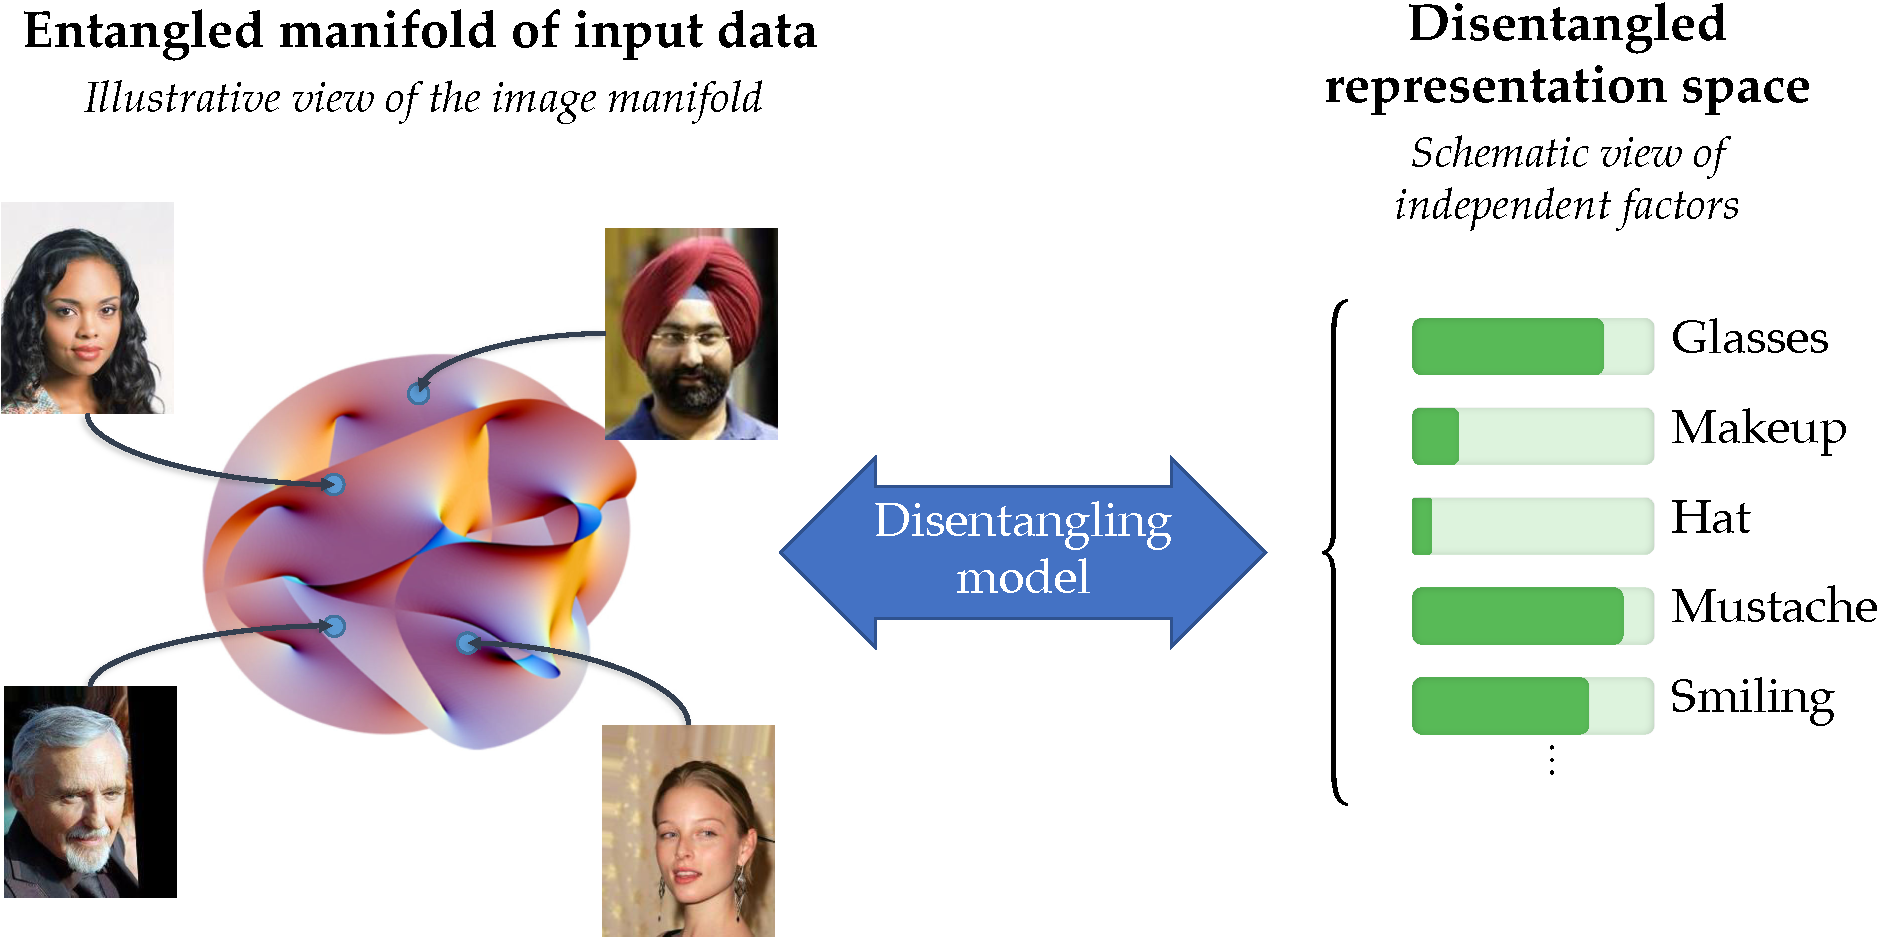
\includegraphics[width=0.9\textwidth]{images/shade_disentangling}
    \titlecaption{Illustration of the purpose of disentangling}{Here, the disentangling model provides a bijective mapping between a complex entangled manifold of faces and a series of independant semantic attributes.}
    \label{shade:fig:disentangling}
\end{figure}

When trying to further improve the quality of the representations of \acp{DNN} arises the question of \textit{disentangling}. This problem can encompass a large range of techniques, but the general principle is to propose models that produce representations that separate well the different factors of variation of the dataset. We illustrate this idea in \autoref{shade:fig:disentangling}. Since the definition of disentangling \citep{higgins2018towards} and what the ``factors of variation'' are for a given dataset are both vague, they can vary widely from one method to the other which thus makes for a very broad literature.

A first category of techniques are simple generative models ($G(\vy, \vhz)$) that combine and separate a binary class information $\vy$ from the rest of the information (non-class related) stored in $\vhz$. While initial work relied on a natural tendency of the model to separate the information \citep{cheung2014discovering,perarnau2016invertible}, more recent models explicitly try to make the model remove class information from $\vhz$ \citep{Lample2017,Liu2018}.

However, representing each factor by a binary representation is very constraining and limiting because factors often comprise internal variability that we would like to model. Thus a sort of variation on those generative models propose to better represent and separate the information by learning two complementary latent representations $\vhy$ and $\vhz$, one for the class $\vy$ and one for non-class related attributes $\vz$. A famous contribution by \citet{Mathieu2016} propose this sort of technique, using adversarial learning \citep{Goodfellow2014} to separate the information. It was later followed by many extensions of this idea to better represent those factors of variation \citep{peng2017reconstruction,Jaiswal2018,Liu2018a}.

Finally, another category of methods propose to find and separate factors of variation without any label, an approach we could call unsupervised disentangling. In this case, the training objective mostly focuses on finding statistically independent representations that can also be used to reconstruct the input data. Many of those methods are based on the $\beta$-\acs{VAE} \citep{higgins2017beta,chen2018isolating}, which proposes to increase the independence of the neurons in the latent space $\vh$ of a \acs{VAE}. The main issue with this type of models is that without any labels, it is impossible to ensure that semantic factors of interest will in fact be represented and separated as we would hope they do.

Being able to disentangle independent factors of variation is an important research direction for \ac{DL}, producing more interpretable and reliable latent representations. This is why we will address this problem more deeply in \autoref{chapter:dualdis} and propose a new approach that separates and structures the information in the latent space.

\section{SHADE: Encouraging Invariance in DNNs} \label{shade:sec:model}

As we saw in \autoref{shade:sec:RW_regul}, many solutions exist to regularize \acp{DNN} and improve their generalization performance. In particular, adding invariance in the representations of \acp{DNN} is a promising and well addressed solution, especially for classification purposes.
%
Indeed, finding invariant representations has long been an important goal in \acf{CV}, as illustrated by the famous \acf{SIFT} descriptors used before \acf{DL}. 
%
We have seen that recent solutions using invariance try to model the transformations a representation should be invariant to, for example, \acf{DA} will add invariance toward handcrafted factors like rotation, scale, Gaussian noise, \etc; and this is also the case for architectural blocks (\eg translation invariance for max-pooling) and invariant architectures (\eg rotation invariance for \citep{dieleman2015rotation}).

However, for image recognition, it is very difficult to design an explicit modeling of all transformations a model should be invariant to.
%
Thus, for our first contribution, we propose to work on the discriminative quality of the representations produced by a \ac{DNN} by working on the invariance properties of those representations.
%
In particular, we want to let the network find what \textit{kind} of invariance should be produced by the model, using an entropy-based measure as a surrogate for invariance.

Indeed, as we have seen at the end of \autoref{shade:sec:RW_regul_loss}, the \acf{IB} framework is a recent and interesting source of inspiration to design new regularization methods for \ac{DL}. Based on this idea, we propose a regularizer called \textbf{\acf{SHADE}} that aims at improving the intra-class invariance of the representations produced by the model. Our main motivation is to design a model that is robust to variations in the training data while preserving class information. Because of this, our regularizer minimizes the entropy of the representations $\Y$ conditionally to a class $\C$:
\begin{equation}
    \min \Ent(\Y \mid \C)\,.
\end{equation}

In this section, we will detail the motivations of using conditional entropy to measure the invariance of the representations. We then develop a differentiable and tractable expression of this \ac{SHADE} criterion. Finally, we evaluate its ability to regularize a large variety of architectures, on CIFAR-10 and ImageNet; and when using datasets with a small number of samples.

\subsection{Context}

    \paragraph{Notations and definitions.} For our work using information theory, we use the following random variables and notations. We consider a random variable input $X\in \mcX$ associated to a target class variable $\C \in \mcY= \{1,2,..,N_\mathrm{cls}\}$. $X$ is fed to a \ac{DNN} named $E$ (for encoder) of parameters $\vw$ producing a succession of intermediate representations $\Y_\ell$ after each layer $\ell$; $\Y$ designating any of those representations.
    We will also use information theory measures. First, the Shannon entropy noted $\Ent$ \citep[\cf\unskip][]{element}. Second, the mutual information noted $\IM$, which quantifies the amount of information shared between two random variables. Considering $U \in \mcU$ and $V\in \mcV$ with respective marginal probability distributions $P_U$ and $P_V$ and mutual distribution $P_{(U,V)}$, we have:
    \begin{equation}
        \IM(U,V) = \int_{\mathcal{U}\times\mathcal{V}}P_{(U,V)}(u,v)\log\bigg[\frac{P_{(U,V)}(u,v)}{P_U(u)P_V(v)}\bigg] \dd u \dd v
    \end{equation}
    Useful properties between the two measures are:
    \begin{equation}
        \IM(U,V) = \IM(V,U) = \Ent(U) - \Ent(U\mid V) = \Ent(V) - \Ent(V\mid U)
    \end{equation}

    \paragraph{\acf{IB}.} The \acf{IB} framework proposes to regularize the encoder $E$ by optimizing the following objective:
    \begin{equation}
        \begin{cases}
        \max_{\vw} & \IM(\Y, \C)\\
        \text{s.t.} & \IM(X, \Y) < D
        \end{cases}
    \end{equation}
    %
    This can be rewritten with a Lagrange multiplier $\beta$ as:
    \begin{equation}
        \max_{\vw}\, \IM(\Y, \C) - \beta \IM(X, \Y) \,.
    \end{equation}
    %
    In this optimization problem, the first term $\IM(\Y, \C)$ maximizes the mutual information between the representation and the target, which can be interpreted as equivalent to the usual classification training objective minimizing cross-entropy between $\vyh$ and $\vy$. The second term $-\IM(X, \Y)$ minimizes the mutual information between the input and the representation, making the model forget most of the information. Indeed, ideally, the model should filter out most of the input information that is useless and focus only on the information that is related to the target $\C$.

    \subsection{Measuring Invariance with Conditional Entropy} \label{shade:sec:intuition}

    Inspired by this \ac{IB} framework, we propose to analyze in more details why we propose to use entropy, and more precisely conditional entropy, as a measure of the invariance that we want to encourage.

    \begin{figure}[tb]
        \begin{subfigure}[t]{\linewidth}
            \centering
            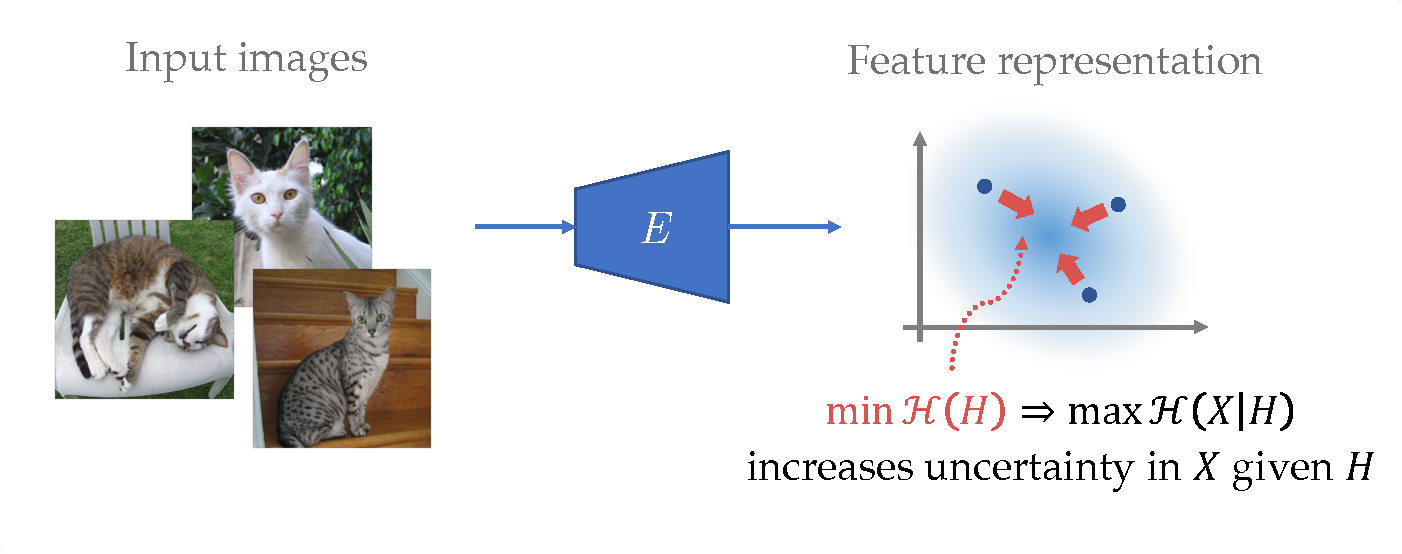
\includegraphics[width=0.9\linewidth]{images/shade_entropy}
            \vspace{0.7em}
            \titlecaption{Effect of minimizing $\Ent(\Y)$}{Representations get more similar, increasing the entropy of the input given the representation and thus the invariance.}
            \label{shade:fig:entropy:reg}
        \end{subfigure}
        
        \begin{subfigure}[t]{\linewidth}
            \centering
            \vspace{1.2em}
            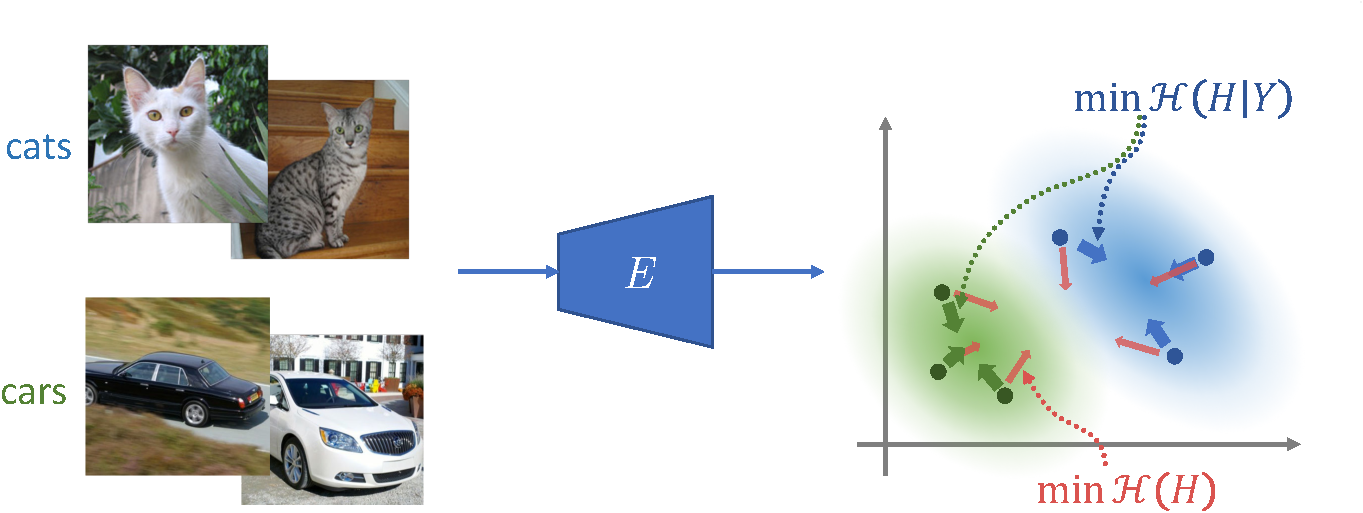
\includegraphics[width=0.9\linewidth]{images/shade_condentropy}
            \vspace{0.7em}
            \titlecaption{Effect of minimizing $\Ent(\Y\mid \C)$}{Representations get more similar for each class independently, making the representations more invariant \textit{intra-class}.}
            \label{shade:fig:entropy:cond}
        \end{subfigure}
        \titlecaption[c]{Illustration of the effect of entropy minimization}{ and the difference between normal and conditional entropy as a regularizer.}
        \label{shade:fig:entropy}
    \end{figure}

    \paragraph{Entropy as a measure of invariance.}
    
        First, to study how the entropy of a representation $\Ent(\Y)$ can be interpreted as a measure of the invariance of the representations of a model, let's write:
        \begin{equation}
            \Ent(\Y) = \IM(X,\Y) + {\Ent(\Y \mid X)} \,.
        \end{equation}
        Considering that our encoder $E$ is a deterministic mapping of $X$ into $H$ (\ie a model without stochastic noise), we know that $\Ent(\Y\mid X)=0$, therefore:
        \begin{equation}
            \Ent(\Y) = \IM(X, \Y) = \Ent(X) - \Ent(X \mid \Y)\,.
        \end{equation}
        
        $\Ent(X)$ is the entropy of the data and is fixed, therefore, $\Ent(\Y)$ is inversely related to $\Ent(X\mid \Y)$. This entropy $\Ent(X\mid \Y)$ is a good measure to quantify how invariant a representation is. Indeed, if a representation is invariant to many changes in the image, this means that many inputs have the same representation. Consequently, given a representation sample, it will be difficult to guess from which input it has been computed. These properties are perfectly captured by $\Ent(X\mid \Y)$, representing the uncertainty in the input $X$ knowing a representation $\Y$. The bigger the uncertainty, the harder it is to predict $X$. The schematic behavior of a model on which we minimize $\Ent(\Y)$ is represented in \autoref{shade:fig:entropy:reg}, where representations are made more and more similar. Formally, when trying to guess $X$ knowing $\Y$, we can lower bound the error made in the best case, with an increasing function of the conditional entropy \citep[Appendix D]{Blot2018full}. % as developed in Appendix \ref{shade:sec:reconstr_err}.
        Therefore, it seems that $\Ent(\Y)$ is a good measure of the invariance of the model.
        
        In the particular case of \acf{DL}, \citet{resnet}, proposing ResNet, explain that the stacking of multiple layers is responsible for improving the generalization of \acp{DNN}. This fact can be explained by the data processing inequality \citep{element}. This states that in the case of finite input space, each additional computation layer can only remove a certain amount of information and cannot add any. As clearly illustrated in \citet{IBdeep}, for each stage, the representation has a lower entropy than the representation of the preceding layer. Increasing the depth increases the capacity of the network to reduce the overall entropy of the \ac{DNN} representation thus increasing their invariance.

    \paragraph{Importance of conditional entropy.}
        We have seen that lowering the entropy of the representation enables to make it more invariant. However, another fact reported by \citet{resnet} is that stacking layers increases the difficulty to train the network. Indeed, when reducing too much the entropy, there is a risk that the information about the label is filtered as well.  The representation is so invariant that it is no longer possible to distinguish between the classes.
        In \citet{resnet}, they solve this issue by forcing the transmission of additional information through skip-connections while IB prescribes to maximize the compression rate at constant information about the label. All this highlights the fact that having invariant representations is interesting if it is intra-class invariant.

        Indeed, in our case above, we focused on a too broad meaning of invariance that could lead to some issue. We stated that we want to be invariant to any kind of information from the input $X$, which is actually not true.        
        In fact, we want to keep information regarding the label of the input. To illustrate, we do not want two inputs from different classes to have the same representation, but do not matter if inputs from the same class have the same representation. This is why we prefer to focus on a criterion quantifying the intra-class compression rate in order to maximize intra-class invariance: $\Ent(\Y\mid \C)$. This is schematized in \autoref{shade:fig:entropy:cond} that shows the difference between conditional and non-conditional entropy on representations.
        
        \begin{figure}[tbp]%{0.49\textwidth}
            \centering
            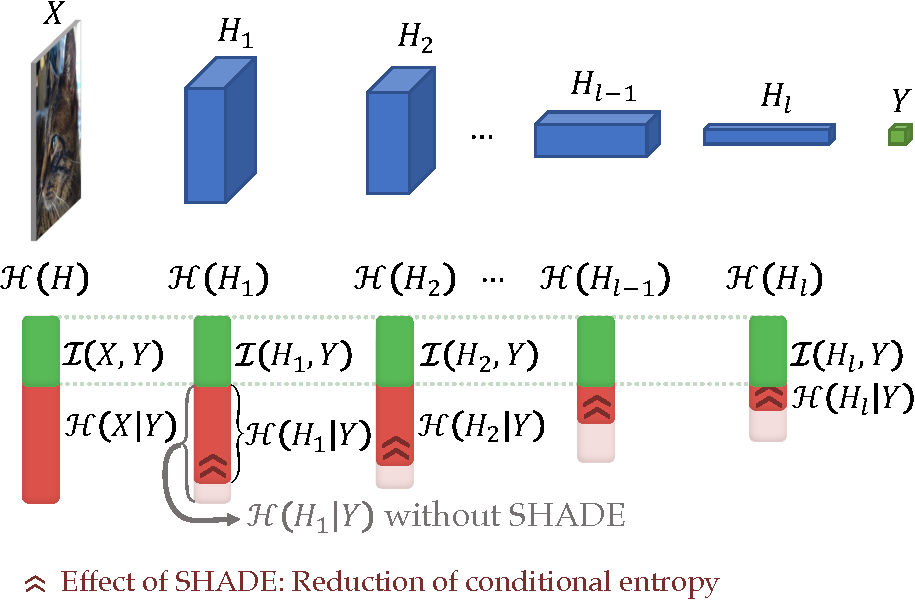
\includegraphics[width=0.7\textwidth]{images/shade_motivation}
            \titlecaption{Illustration of the effect of \acs{SHADE}}{Considering a \acs{DNN} architecture with corresponding layers' entropies, we show the layer-wise action of \acs{SHADE}. Given that $\Ent(\Y_\ell) = \IM(\Y_\ell,\C)+\Ent(\Y_\ell\mid \C)$, \acs{SHADE} minimizes $\Ent(\Y_\ell\mid \C)$ without affecting $\IM(\Y_\ell,\C)$.}
            \label{shade:fig:motivation}
        \end{figure}    

        \paragraph{Behavior of \ac{SHADE} and comparison with \ac{IB}.} Our criterion $\Ent(\Y\mid \C)$ therefore differs from standard \ac{IB} regularizers based on $\IM(X, \Y)$
        \citep[\eg\unskip][]{Achille2016, IBvariational}.
        In fact, the mutual information minimized in \ac{IB} can be rewritten:
        \begin{equation}\label{shade:eq:IB}
            \IM(X, \Y) = \Ent(\Y\mid \C) + \IM(\C, \Y) \,.
        \end{equation}
        Thus, we see that our choice of optimizing only $\Ent(\Y\mid \C)$ ignores the term $\IM(\C, \Y)$.  In fact, we argue that removing $\IM(\C, \Y)$ from the optimization is a good thing since this term is analogous to the classification loss and should not be minimized since it would be detrimental to the actual objective.
        When minimizing $\IM(X, \Y)$, there is no control over how both terms $\Ent(\Y\mid \C)$ and $\IM(\C, \Y)$ are affected. 
        Our regularizer is therefore beneficial in the sense that minimizing $\Ent(\Y\mid \C)$ does not conflict with  the mutual information $\IM(\C, \Y)$ between the representation and the label, information useful for classification that should not be penalized.

        The behavior of \ac{SHADE} is illustrated in \autoref{shade:fig:motivation}, where we show for each layer of a \ac{DNN} this decomposition of the information $\Ent(\Y)$ into the desired information $\IM(\C, \Y)$ used for classification, and the information \ac{SHADE} intends to minimize $\Ent(\Y\mid \C)$. Next, we will further describe the development \ac{SHADE}, our regularization term based on the conditional entropy $\Ent(\Y\mid \C)$ designed to drive the optimization toward more intra-class invariant representations.

 \subsection{Entropy-based Regularization for Deep Neural Networks} \label{shade:sec:dev}
 \label{shade:sec:noncond_entropy}

    We now propose to describe how we develop and instantiate our \ac{SHADE} regularizer. This section will present the important choices that we make to obtain the loss function for \ac{SHADE}, all the details about this process are given in \autoref{chapter:shadeA}.

        \paragraph{Toward a unit-wise regularization.}
        
        Considering a \ac{DNN} composed of $L$ layers that transform sequentially the input, we first propose to regularize all the layers independently and minimize the sum of entropies $\Omega_{\mathrm{layers}} = \sum_{\ell = 1}^L \Ent(\Y_\ell \mid \C)$.
        
        Noting $\Y_{\ell,i}$ the unit neurons of $\Y_{\ell}$, we propose to use the  upper bound $\Ent(\Y_\ell \mid \C) \le \sum_{i=1}^{D_\ell} \Ent(\Y_{\ell,i} \mid \C)$ to define a unit-wise criterion that \ac{SHADE} will seek to minimize. Since we only work on individual and independent neurons, we will use the notation $\Y$ instead of $\Y_{\ell,i}$ for simplicity in the rest of the chapter. We thus seek to minimize:
            \begin{equation}
                \Omega_{\mathrm{units}} = \sum_{l=1}^L \sum_{i = 1}^{D_\ell} \underbrace{\Ent(\Y \mid \C)}_{\omega_{\mathrm{unit}}(\Y\mid \C)} \,.
            \end{equation}

        \paragraph{Limitations.}
        
            Finding a tractable and differentiable expression of $\Ent(\Y\mid \C)$ is not obvious for multiple reasons.
            The conditional entropy $\Ent(\Y\mid \C)$ requires to compute $N_\mathrm{cls}$ different entropies $\Ent(\Y\mid \C_k)$, which, when working on batches, reduces the number of samples used to compute each entropy down to problematic levels. Entropy estimators are also very inaccurate with few samples and require a discretization of the space using a histogram, an operation that raises new issues on how to do it and to keep it tractable since bins for each neuron would lead to important memory usages.
        
        \paragraph{Reducing complexity with a binary latent code.}

            Considering a neuron $\Y$ prior to the non-linearity, the \acs{ReLU} can be interpreted as making it act as a detector, returning a signal when a certain pattern is present in the input. We thus propose to associate a binomial variable $Z$ to each unit variable $\Y$ (before \acs{ReLU}). This variable $Z$ indicates if a particular pattern is present in the input ($Z=1$ when $\Y \gg 0$) or not ($Z=0$ when $\Y \ll 0$).
            
            We then assume that this variable $Z$ is a sufficient statistic \citep[see definition by][]{element} of $H$ for $\C$, \ie that it contains the necessary information from $H$ to predict the class $\C$. This means that we have $\IM(\Y, \C) = \IM(\Y, Z)$ and we get the equivalent equality $\Ent(\Y\mid \C)= \Ent(\Y\mid Z)$. This has the advantage of requiring to compute only 2 entropies ($Z=0$ and $1$) instead of $N_\mathrm{cls}$. We finally obtain:
            \begin{equation}
                \omega_{\mathrm{unit}}(\Y\mid \C) = \Ent(\Y\mid \C)= \Ent(\Y\mid Z) = \sum_{z\in\{0,1\}} p(z) \Ent(\Y\mid Z=z).
            \end{equation}

            This variable $Z$ represents a semantically meaningful factor about the class $\C$ and from which the input $X$ is generated, and $\Y$ is a quantification of the possibility for this semantic attribute $Z$ to be present in the input or not. Interpreting $p(Z \mid \Y)$ as the probability of presence of the semantic attribute in the input, we choose to define it as:
            \begin{equation}
                \begin{cases}
                    p(Z=1\mid H) = \sigma(H) \\ p(Z=0 \mid H) = 1- \sigma(H)
                \end{cases}
                \  \text{using the sigmoid function } \sigma(H) = \frac{1}{1 + e^{-H}}.
            \end{equation}
            
            
        \paragraph{Using a variance bound for tractability.}

            To solve the problem of the complexity of estimating the entropies, we propose to use a simple bound on $\Ent(\Y\mid Z)$ using the variance, which does not require the definition of a histogram:
            \begin{equation}
                \label{shade:variancebound}
                \Ent(\Y \mid Z) \le \frac{1}{2}\ln\big(2 \pi e \var(\Y\mid Z)\big).
            \end{equation}
            
            This bound converges well and should be very tight if we consider that activations approximately follow a Gaussian distribution, which is often the case. We then propose to simplify the expression and only keep the simpler term $\var(\Y\mid Z)$. We then estimate our loss using Monte-Carlo sampling on $K$ inputs, and use a moving average on the neurons to estimate the expectancy $\mu^z = \EE(\Y\mid z)$ to compute this variance. We thus obtain our final loss for \ac{SHADE}:
            \begin{align}
                \Omega_\mathrm{SHADE} &= \sum_{\ell=1}^{L}\sum_{i=1}^{D_\ell}\sum_{z \in \{0,1\}} p(Z_{\ell,i} = z \mid \Y) \var(\Y\mid Z_{\ell,i}=z)\,; \\
                \Aboxed{
                \Omega_{\mathrm{SHADE}} &= \sum_{\ell=1}^{L}\sum_{i=1}^{D_\ell}\sum_{k=1}^K \sum_{z \in \{0,1\}} p\left(Z_{\ell,i} = z\,\middle|\, \Y_{\ell,i}^{(k)}\right) %\times \\[-3mm]
                \left({\Y_{\ell,i}^{(k)}} - \mu_{\ell,i}^ z\right)^2\,.}
            \end{align}
    
    We obtain a regularizer that is applied on each neuron of the network, that is differentiable, tractable and that can be integrated into the usual optimization process of a \ac{DNN}. Notably, \ac{SHADE} requires only a small amount of  additional computation and memory usage (computation and storage of two moving averages per neuron). For comparison, \ac{SHADE} adds only half as many parameters as \acf{BN} does.
    

    \subsubsection*{Comparison to Non-conditional Entropy and relation to Weight Decay}

    We propose to compare \ac{SHADE} to a variant based on optimizing the entropy of the representations $\Ent(\Y)$ instead of $\Ent(\Y\mid\C)$.
    For this, one can use a variance bound similar to \autoref{shade:variancebound}: $\Ent(\Y) \le \nicefrac{1}{2}\ln(2 \pi e \var(\Y))$ to derive a loss in order to minimize the representations' entropy $\Ent(\Y)$. Thus, minimizing the variance of the representations is an upper bound of the entropy. This can be done by penalizing the empirical variance, using an alternative loss called \textit{VarEntropy}, constructed the same way SHADE has been derived, but avoiding the introduction of a latent variable $Z$:
    \begin{equation}
        \label{shade:eq:varreg}
        \Omega_{\mathrm{VarEntropy}} =  \frac{1}{K}\sum_{k=1}^K \big(H^{(k)}- \EE(\Y)\big)^2 \,.
    \end{equation}

    Interestingly, we can show that the weight decay actually reduces this variance $\var(\Y)$ and therefore $\Ent(\Y)$ under some conditions. In fact when $\Y = \vw^\top X + \bb$, by estimating $\Lambda = \cov(X)$, the variance takes the immediate form $\var(\Y) = \vw^{\top} \Lambda \vw$. If $\Lambda = I\!d$ --\,the identity matrix\,--, meaning that the input coordinates are considered independent and with unit variance, then $\var(\Y)= ||\vw||_2^2$. It corresponds to the weight decay regularization or $L_2$ penalty. Even if within a \ac{DNN} layer, \acf{BN} tends to enforce this unit variance hypothesis and the depth of \ac{DNN} tends to ensure the independence hypothesis the weight decay remains poor at improving generalization as illustrated in \citet{rethinking}.



\subsection{Evaluation}
\label{shade:sec:expes}

We now propose different experiments to validate the capability of \ac{SHADE} to regularize common \acf{CV} architectures. First, classification results on CIFAR-10 for different architectures to show that \ac{SHADE} is able to regularize a broad range of models. We also validate that our regularization can be applied on large scale models and datasets by applying it on ImageNet. We then investigate the behavior of \ac{SHADE} when using few images before some more in-depth analysis of the behavior of \ac{SHADE} and its intuitions.

    \subsubsection{Image Classification with Various Architectures on CIFAR-10}
    \label{shade:sec:cifar10}
    
    \begin{table}[t]
            \centering
            \begin{tabular}{lccccc}
            \toprule
                            & MLP & AlexNet & ResNet & Inception\\
            \midrule
            No regul.        & 62.38 & 83.25 & 89.84 & 90.97 \\
            Weight decay     & 62.69 & 83.54 & 91.71 & 91.87 \\
            VarEntropy       & 63.70 & 83.61 & 91.72 & 91.83 \\
            Dropout          & 65.37 & 85.95 & 89.94 & 91.11 \\
            \cmidrule{1-5}
            SHADE            & 66.05 & 85.45 & \textbf{92.15} & \textbf{93.28}\\
            SHADE + Dropout  & \textbf{66.12} & \textbf{86.71} &  92.03 &  92.51\\
            \bottomrule
            \end{tabular}
            \titlecaption[c]{Classification accuracy (\%) on CIFAR-10}{test set.}
            \label{shade:accuracies}
        \end{table}
         
        First, we perform image classification on the CIFAR-10 dataset, which contains 50k training images and 10k test images of 32$\times$32 RGB pixels, fairly distributed within 10 classes \citep{cifar}. Following the architectures used by \citet{rethinking}, we use a three-layer \acf{MLP}, and an AlexNet-like model with 3 convolutional and 2 fully connected layers and a small Inception model. We also use a ResNet architecture from \citet{wideresnet}. Those architectures represent a large family of \ac{DNN} and some have been well studied in \citet{rethinking} regarding their generalization ability. For training, we use randomly cropped images of size 28$\times$28 with random horizontal flips. For testing, we simply center-crop 28$\times$28 images. We use momentum SGD for optimization \citep[same protocol as][]{rethinking}.
           
        We compare \ac{SHADE} with three regularization methods, namely {\em weight decay}, {\em dropout} and {\em VarEntropy} presented in \autoref{shade:eq:varreg}. For all architectures, the regularization parameters have been cross-validated to find the best ones for each method and the obtained accuracies on the test set are reported in \autoref{shade:accuracies}.
        
        We obtain the same trends as \citet{rethinking}, which get a small improvement of 0.31\% with weight decay on AlexNet. The improvement with weight decay is slightly more important with ResNet and Inception (0.87\% and 0.90\%) probably thanks to the use of \acf{BN}. In our experiments, dropout improves generalization performances only for AlexNet and \ac{MLP}. It is known that the use of \ac{BN} lowers the benefit of dropout, which is in fact not used in \citet{resnet}.
        
        We first notice that for all kind of architectures the use of \ac{SHADE} significantly improves the generalization performance. It demonstrates the ability of \ac{SHADE} to regularize the training of deep architectures. Moreover, \ac{SHADE} systematically outperforms other regularizations of the same type such as weight decay or VarEntropy, illustrating the advantage of minimizing the conditional entropy instead of the entropy directly. 
        
        Finally, \ac{SHADE} shows better performances than dropout on all architecture except on AlexNet, for which they seem to be complementary, probably because of the very large number of parameters in the fully-connected layers, with best performances obtained with \ac{SHADE} coupled with dropout. This association is also beneficial for \ac{MLP}. On Inception and ResNet, even if dropout and \ac{SHADE} independently improve generalization performances, their association is not as good as \ac{SHADE} alone, probably because it enforces too much regularization.
    
            
    \subsubsection{Large Scale Classification on ImageNet}
    \label{shade:imagenetExperiment}

        \begin{table}[t]
            \centering
            \begin{tabular}{lcc}
            \toprule
                                & \multicolumn{2}{c}{Accuracy (\%)} \\
                                & Top-1   & Top-5   \\
            \midrule
            ResNet-101       & 77.56\% & 93.89\% \\
            WELDON           & 78.51\% & 94.65\% \\
            WELDON + SHADE   & \bfseries 80.14\% & \bfseries  95.35\% \\
            \bottomrule
            \end{tabular}

            \titlecaption[c]{Classification accuracy (\%) on ImageNet}{validation set.}
        \label{shade:tab:imagenet}
        \end{table}

        In order to experiment \ac{SHADE} regularization on very large scale dataset, we train on ImageNet \citep{imagenet} a WELDON network from \citet{weldone} adapted from ResNet-101. This architecture changes the forward and pooling strategy by using the network in a fully-convolutional way and adding a max+min pooling, thus improving the performance of the baseline network.
        
        There are two differences between the two networks: first, for WELDON the images are simply re-scaled to size 448$\times$448 before being forwarded into the network; second, compared to ResNet-101 architecture, the final average pooling and fully connected layer are replaced with a 1$\times$1 convolutional layer and a particular max+min pooling described in \citet{weldone}. This layer averages the 50 highest and 50 lowest activations of the 14$\times$14 output feature map to give a prediction.

        Results are summarized in \autoref{shade:tab:imagenet}. We report the results of a pre-trained ResNet-101 and the WELDON architecture using those weights. After fine-tuning the network using \ac{SHADE} we obtain an improvement over the WELDON baseline, demonstrating the ability to apply \ac{SHADE} on very large scale image classification successfully. 
    
       
    \subsubsection{Training with a Limited Number of Samples}
        
        \begin{figure}[tb]
            \centering
            \begin{subfigure}[t]{0.49\textwidth}
                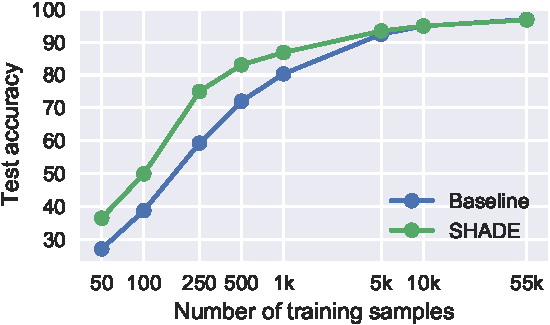
\includegraphics[width=\textwidth]{images/shade_MNISTM_reguls.pdf}
                \caption{Results for MNIST-M.}
                \label{shade:fig:limited_mnistm}
            \end{subfigure}%
            ~
            \begin{subfigure}[t]{0.49\textwidth}
                 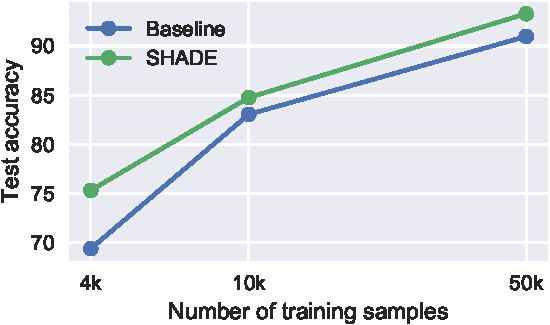
\includegraphics[width=\textwidth]{images/shade_CIFAR10_reguls.pdf}
                \caption{Results for CIFAR-10.}
                \label{shade:fig:limited_cifar10}
            \end{subfigure}
            
            \vspace{5mm}
            \begin{subfigure}[t]{0.85\textwidth}
                \centering
                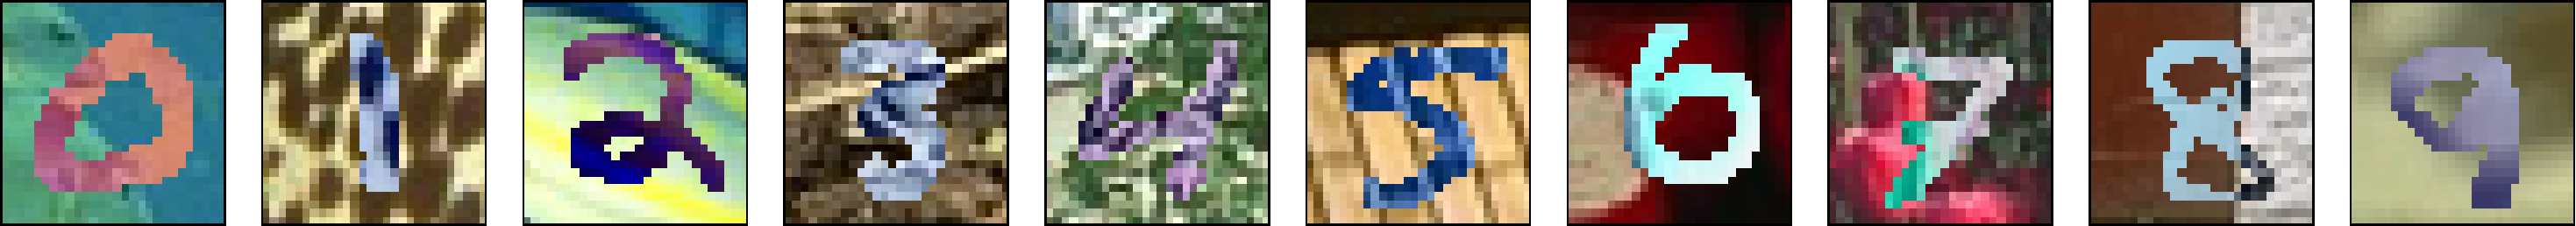
\includegraphics[width=\textwidth]{images/shade_MNISTM_samples.pdf}
                \caption{Examples of MNIST-M images misclassified by the baseline and correctly classified using SHADE, both trained with 250 samples.}
                \label{shade:fig:limited_mnistm_viz}
            \end{subfigure}
            
            \titlecaption[c]{Results when training with a limited number of samples}{in the training set for MNIST-M and CIFAR-10 with and without SHADE.}
            \label{shade:fig:limited_dataset}
        \end{figure}
        
        When datasets are small, \acp{DNN} tend to overfit quickly and regularization becomes essential. zBecause it tends to filter out information and make the network more invariant, \ac{SHADE} seems to be well fitted for this task. To investigate this, we propose to train \acp{DNN} with and without \ac{SHADE} on CIFAR-10 and MNIST-M with different numbers of samples in the training set.
        
        First, we tested this approach on the digits dataset MNIST-M \citep{ganin2015unsupervised}. This dataset consists of the MNIST digits where the background and digit have been replaced by colored and textured information (see \autoref{shade:fig:limited_mnistm_viz} for examples). The interest of this dataset is that it contains lots of unnecessary information that should be filtered out, and is therefore well adapted to measure the effect of \ac{SHADE}.
        
        We train a simple \ac{ConvNet} (3 convolutional layers with pooling and 1 fully connected layer) with different numbers of samples of MNIST-M. The samples, chosen uniformly in the classes for each value of $N$, are kept the same for the baseline and \ac{SHADE}. The results can be seen in \autoref{shade:fig:limited_mnistm}. We can see that especially for small numbers of training samples ($<$ 1000), \ac{SHADE} provides an important gain of 10 to 15\% points over the baseline. This shows that SHADE helped the model in finding invariant and discriminative patterns using fewer data samples.
        
        Additionally, \autoref{shade:fig:limited_mnistm_viz} shows samples that are misclassified by the baseline model but correctly classified when using \ac{SHADE}. These images contain a large amount of intra-class variance (color, texture, etc.) that is not useful for the classification tasks. By encouraging the model to discard information, \ac{SHADE} obtains an important performance gain on this dataset and especially when only few training samples are given.
        
        Finally, to confirm this behavior, we also applied the same procedure in a more conventional setting by training an Inception model on CIFAR-10. \autoref{shade:fig:limited_cifar10} shows the results in that case. We can see that once again SHADE helps the model gain in performance and that this behavior is more noticeable when the number of samples is limited, allowing a gain of 6\% when using 4000 samples.

    \subsection{Discussion of SHADE}

    With \ac{SHADE}, we introduced a new regularization method for \acp{DNN} training that focuses on minimizing the entropy of the representation conditionally to the labels.
    
    Inspired by the \acf{IB} framework, we proposed to increase the invariance of the representations of \acp{DNN} without any prior model on the factors to which those representations should be invariant and let the model find those factors. Thus, \ac{SHADE} is able to increase the intra-class invariance of the model while keeping class information.

    To develop \ac{SHADE}, we make some hypotheses that we validate in additional experiments described in \autoref{chapter:shadeA}. First, we diverge from the regular \ac{IB} framework as described in \autoref{shade:eq:IB} because we show that part of the mutual information $\IM(X,H)$ is important for classification, as validated in \autoref{shadeA:sec:exp_cond}. We also assume that neurons of a \ac{DNN} act as a binary detector of factors that encode the class information, a hypothesis that we validate in \autoref{shadeA:sec:exp_latent}.

    We also showed that \ac{SHADE} significantly outperforms standard approaches such as weight decay or dropout with various \ac{DNN} architectures on CIFAR-10. We also validated the scalability of \ac{SHADE} by applying it on ImageNet. 
    The invariance potential brought out by {SHADE} is further illustrated by its ability to ignore irrelevant visual information (texture, color) on MNIST-M. We also highlight the increasing benefit of our regularizer when the number of training examples becomes small.
 
\section{Conclusion}

    In this chapter, we introduced the recent development in the domain of \acf{DL} and in particular with \acfp{ConvNet}. We saw that deep convolutional architectures are now ubiquitous in \acf{CV} research and produce impressive results. To reach these performances however, because of their complexity, a key aspect of research focus on proposing regularization techniques that are required to make those architectures generalize well to unseen data. As we have seen, many possible regularization approaches exist, in particular by adding new data, changing the structure of the model or adding loss terms to enforce constraints on the model.

    Our first contribution in this thesis consisted in proposing a new regularization method called \ac{SHADE}, that takes the form of a new loss. Inspired by the \acf{IB} framework, \ac{SHADE} influences the representations of a \acp{ConvNet} to be more invariant to the variance in visual inputs conditionally to the class. \ac{SHADE} thus makes the representations more intra-class invariant and allows to obtain better classification results, as we demonstrated by using many \ac{DNN} architectures with \ac{SHADE} on CIFAR-10 but also on ImageNet.

    Another important direction to improve \acp{DNN} lies in the possibility of using additional unlabeled data, which could greatly help the generalization performances for a low cost compared to producing new labeled data. \acf{SSL} techniques address this issue, often by mixing regularization ideas adapted to discriminative models with motivations similar to the ones of \ac{SHADE}; and generative properties with models that are able to encode an image and decode its representation back into the image. In this case, an invariance regularization like \ac{SHADE} would conflict with this second goal. To solve this conflict, it is possible to work on the architecture of the model and go beyond the usual basic one-branch encoder-decoder architecture. This idea will be further developed in \autoref{chapter:hybridnet} where we propose a new type of architecture to address this issue.

    Finally, we also saw that designing \acp{ConvNet} that produce disentangled representations of the different factors of variation of the data is an interesting direction to improve the semantic quality of those models, making them both more powerful for other tasks and more interpretable. To further work on this idea of structuring the information of deep \acp{ConvNet}, in \autoref{chapter:dualdis}, we address the problem of disentangling by proposing a new architecture that separates the information in a structured dual latent space for image editing and data generation.
